% Options for packages loaded elsewhere
\PassOptionsToPackage{unicode}{hyperref}
\PassOptionsToPackage{hyphens}{url}
\PassOptionsToPackage{dvipsnames,svgnames,x11names}{xcolor}
%
\documentclass[
  letterpaper,
  DIV=11,
  numbers=noendperiod]{scrartcl}

\usepackage{amsmath,amssymb}
\usepackage{iftex}
\ifPDFTeX
  \usepackage[T1]{fontenc}
  \usepackage[utf8]{inputenc}
  \usepackage{textcomp} % provide euro and other symbols
\else % if luatex or xetex
  \usepackage{unicode-math}
  \defaultfontfeatures{Scale=MatchLowercase}
  \defaultfontfeatures[\rmfamily]{Ligatures=TeX,Scale=1}
\fi
\usepackage{lmodern}
\ifPDFTeX\else  
    % xetex/luatex font selection
\fi
% Use upquote if available, for straight quotes in verbatim environments
\IfFileExists{upquote.sty}{\usepackage{upquote}}{}
\IfFileExists{microtype.sty}{% use microtype if available
  \usepackage[]{microtype}
  \UseMicrotypeSet[protrusion]{basicmath} % disable protrusion for tt fonts
}{}
\makeatletter
\@ifundefined{KOMAClassName}{% if non-KOMA class
  \IfFileExists{parskip.sty}{%
    \usepackage{parskip}
  }{% else
    \setlength{\parindent}{0pt}
    \setlength{\parskip}{6pt plus 2pt minus 1pt}}
}{% if KOMA class
  \KOMAoptions{parskip=half}}
\makeatother
\usepackage{xcolor}
\setlength{\emergencystretch}{3em} % prevent overfull lines
\setcounter{secnumdepth}{-\maxdimen} % remove section numbering
% Make \paragraph and \subparagraph free-standing
\makeatletter
\ifx\paragraph\undefined\else
  \let\oldparagraph\paragraph
  \renewcommand{\paragraph}{
    \@ifstar
      \xxxParagraphStar
      \xxxParagraphNoStar
  }
  \newcommand{\xxxParagraphStar}[1]{\oldparagraph*{#1}\mbox{}}
  \newcommand{\xxxParagraphNoStar}[1]{\oldparagraph{#1}\mbox{}}
\fi
\ifx\subparagraph\undefined\else
  \let\oldsubparagraph\subparagraph
  \renewcommand{\subparagraph}{
    \@ifstar
      \xxxSubParagraphStar
      \xxxSubParagraphNoStar
  }
  \newcommand{\xxxSubParagraphStar}[1]{\oldsubparagraph*{#1}\mbox{}}
  \newcommand{\xxxSubParagraphNoStar}[1]{\oldsubparagraph{#1}\mbox{}}
\fi
\makeatother

\usepackage{color}
\usepackage{fancyvrb}
\newcommand{\VerbBar}{|}
\newcommand{\VERB}{\Verb[commandchars=\\\{\}]}
\DefineVerbatimEnvironment{Highlighting}{Verbatim}{commandchars=\\\{\}}
% Add ',fontsize=\small' for more characters per line
\usepackage{framed}
\definecolor{shadecolor}{RGB}{241,243,245}
\newenvironment{Shaded}{\begin{snugshade}}{\end{snugshade}}
\newcommand{\AlertTok}[1]{\textcolor[rgb]{0.68,0.00,0.00}{#1}}
\newcommand{\AnnotationTok}[1]{\textcolor[rgb]{0.37,0.37,0.37}{#1}}
\newcommand{\AttributeTok}[1]{\textcolor[rgb]{0.40,0.45,0.13}{#1}}
\newcommand{\BaseNTok}[1]{\textcolor[rgb]{0.68,0.00,0.00}{#1}}
\newcommand{\BuiltInTok}[1]{\textcolor[rgb]{0.00,0.23,0.31}{#1}}
\newcommand{\CharTok}[1]{\textcolor[rgb]{0.13,0.47,0.30}{#1}}
\newcommand{\CommentTok}[1]{\textcolor[rgb]{0.37,0.37,0.37}{#1}}
\newcommand{\CommentVarTok}[1]{\textcolor[rgb]{0.37,0.37,0.37}{\textit{#1}}}
\newcommand{\ConstantTok}[1]{\textcolor[rgb]{0.56,0.35,0.01}{#1}}
\newcommand{\ControlFlowTok}[1]{\textcolor[rgb]{0.00,0.23,0.31}{\textbf{#1}}}
\newcommand{\DataTypeTok}[1]{\textcolor[rgb]{0.68,0.00,0.00}{#1}}
\newcommand{\DecValTok}[1]{\textcolor[rgb]{0.68,0.00,0.00}{#1}}
\newcommand{\DocumentationTok}[1]{\textcolor[rgb]{0.37,0.37,0.37}{\textit{#1}}}
\newcommand{\ErrorTok}[1]{\textcolor[rgb]{0.68,0.00,0.00}{#1}}
\newcommand{\ExtensionTok}[1]{\textcolor[rgb]{0.00,0.23,0.31}{#1}}
\newcommand{\FloatTok}[1]{\textcolor[rgb]{0.68,0.00,0.00}{#1}}
\newcommand{\FunctionTok}[1]{\textcolor[rgb]{0.28,0.35,0.67}{#1}}
\newcommand{\ImportTok}[1]{\textcolor[rgb]{0.00,0.46,0.62}{#1}}
\newcommand{\InformationTok}[1]{\textcolor[rgb]{0.37,0.37,0.37}{#1}}
\newcommand{\KeywordTok}[1]{\textcolor[rgb]{0.00,0.23,0.31}{\textbf{#1}}}
\newcommand{\NormalTok}[1]{\textcolor[rgb]{0.00,0.23,0.31}{#1}}
\newcommand{\OperatorTok}[1]{\textcolor[rgb]{0.37,0.37,0.37}{#1}}
\newcommand{\OtherTok}[1]{\textcolor[rgb]{0.00,0.23,0.31}{#1}}
\newcommand{\PreprocessorTok}[1]{\textcolor[rgb]{0.68,0.00,0.00}{#1}}
\newcommand{\RegionMarkerTok}[1]{\textcolor[rgb]{0.00,0.23,0.31}{#1}}
\newcommand{\SpecialCharTok}[1]{\textcolor[rgb]{0.37,0.37,0.37}{#1}}
\newcommand{\SpecialStringTok}[1]{\textcolor[rgb]{0.13,0.47,0.30}{#1}}
\newcommand{\StringTok}[1]{\textcolor[rgb]{0.13,0.47,0.30}{#1}}
\newcommand{\VariableTok}[1]{\textcolor[rgb]{0.07,0.07,0.07}{#1}}
\newcommand{\VerbatimStringTok}[1]{\textcolor[rgb]{0.13,0.47,0.30}{#1}}
\newcommand{\WarningTok}[1]{\textcolor[rgb]{0.37,0.37,0.37}{\textit{#1}}}

\providecommand{\tightlist}{%
  \setlength{\itemsep}{0pt}\setlength{\parskip}{0pt}}\usepackage{longtable,booktabs,array}
\usepackage{calc} % for calculating minipage widths
% Correct order of tables after \paragraph or \subparagraph
\usepackage{etoolbox}
\makeatletter
\patchcmd\longtable{\par}{\if@noskipsec\mbox{}\fi\par}{}{}
\makeatother
% Allow footnotes in longtable head/foot
\IfFileExists{footnotehyper.sty}{\usepackage{footnotehyper}}{\usepackage{footnote}}
\makesavenoteenv{longtable}
\usepackage{graphicx}
\makeatletter
\def\maxwidth{\ifdim\Gin@nat@width>\linewidth\linewidth\else\Gin@nat@width\fi}
\def\maxheight{\ifdim\Gin@nat@height>\textheight\textheight\else\Gin@nat@height\fi}
\makeatother
% Scale images if necessary, so that they will not overflow the page
% margins by default, and it is still possible to overwrite the defaults
% using explicit options in \includegraphics[width, height, ...]{}
\setkeys{Gin}{width=\maxwidth,height=\maxheight,keepaspectratio}
% Set default figure placement to htbp
\makeatletter
\def\fps@figure{htbp}
\makeatother

\KOMAoption{captions}{tableheading}
\makeatletter
\@ifpackageloaded{caption}{}{\usepackage{caption}}
\AtBeginDocument{%
\ifdefined\contentsname
  \renewcommand*\contentsname{Table of contents}
\else
  \newcommand\contentsname{Table of contents}
\fi
\ifdefined\listfigurename
  \renewcommand*\listfigurename{List of Figures}
\else
  \newcommand\listfigurename{List of Figures}
\fi
\ifdefined\listtablename
  \renewcommand*\listtablename{List of Tables}
\else
  \newcommand\listtablename{List of Tables}
\fi
\ifdefined\figurename
  \renewcommand*\figurename{Figure}
\else
  \newcommand\figurename{Figure}
\fi
\ifdefined\tablename
  \renewcommand*\tablename{Table}
\else
  \newcommand\tablename{Table}
\fi
}
\@ifpackageloaded{float}{}{\usepackage{float}}
\floatstyle{ruled}
\@ifundefined{c@chapter}{\newfloat{codelisting}{h}{lop}}{\newfloat{codelisting}{h}{lop}[chapter]}
\floatname{codelisting}{Listing}
\newcommand*\listoflistings{\listof{codelisting}{List of Listings}}
\makeatother
\makeatletter
\makeatother
\makeatletter
\@ifpackageloaded{caption}{}{\usepackage{caption}}
\@ifpackageloaded{subcaption}{}{\usepackage{subcaption}}
\makeatother

\ifLuaTeX
  \usepackage{selnolig}  % disable illegal ligatures
\fi
\usepackage{bookmark}

\IfFileExists{xurl.sty}{\usepackage{xurl}}{} % add URL line breaks if available
\urlstyle{same} % disable monospaced font for URLs
\hypersetup{
  pdftitle={Probability with R - Exercise 1.1},
  pdfauthor={Lucas Liona},
  colorlinks=true,
  linkcolor={blue},
  filecolor={Maroon},
  citecolor={Blue},
  urlcolor={Blue},
  pdfcreator={LaTeX via pandoc}}


\title{Probability with R - Exercise 1.1}
\author{Lucas Liona}
\date{}

\begin{document}
\maketitle

\renewcommand*\contentsname{Table of contents}
{
\hypersetup{linkcolor=}
\setcounter{tocdepth}{3}
\tableofcontents
}

\subsection{Problem}\label{problem}

In a class of 50 students of computing, 23 are female and 27 are male.
The results of their first year Java programming examination are as
follows:

Females: 57, 59, 78, 79, 60, 65, 68, 71, 75, 48, 51, 55, 56, 41, 43, 44,
75, 78, 80, 81, 83, 83, 85 Males: 48, 49, 49, 30, 30, 31, 32, 35, 37,
41, 86, 42, 51, 53, 56, 42, 44, 50, 51, 65, 67, 51, 56, 58, 64, 64, 75
(a) Read these data into R by storing them in the following ways:

As two vectors, one for the females and one for the males. As one
vector, with a factor vector designating the gender.

\begin{enumerate}
\def\labelenumi{(\alph{enumi})}
\setcounter{enumi}{1}
\tightlist
\item
  If it was discovered that the 34th was entered incorrectly and should
  have obtained the marks 46 instead of 86, use an appropriate editing
  procedure to change this.
\item
  Save the workspace in a suitable directory for access later.
\end{enumerate}

Part (a): Reading Data into R First, we'll read the data into R using
the two approaches mentioned in the problem.

\section{Approach 1: Two Separate
Vectors}\label{approach-1-two-separate-vectors}

\begin{Shaded}
\begin{Highlighting}[]
\CommentTok{\# Create separate vectors for female and male scores}
\NormalTok{females }\OtherTok{\textless{}{-}} \FunctionTok{c}\NormalTok{(}\DecValTok{57}\NormalTok{, }\DecValTok{59}\NormalTok{, }\DecValTok{78}\NormalTok{, }\DecValTok{79}\NormalTok{, }\DecValTok{60}\NormalTok{, }\DecValTok{65}\NormalTok{, }\DecValTok{68}\NormalTok{, }\DecValTok{71}\NormalTok{, }\DecValTok{75}\NormalTok{, }\DecValTok{48}\NormalTok{, }\DecValTok{51}\NormalTok{, }\DecValTok{55}\NormalTok{, }\DecValTok{56}\NormalTok{, }\DecValTok{41}\NormalTok{, }\DecValTok{43}\NormalTok{, }\DecValTok{44}\NormalTok{, }\DecValTok{75}\NormalTok{, }\DecValTok{78}\NormalTok{, }\DecValTok{80}\NormalTok{, }\DecValTok{81}\NormalTok{, }\DecValTok{83}\NormalTok{, }\DecValTok{83}\NormalTok{, }\DecValTok{85}\NormalTok{)}
\NormalTok{males }\OtherTok{\textless{}{-}} \FunctionTok{c}\NormalTok{(}\DecValTok{48}\NormalTok{, }\DecValTok{49}\NormalTok{, }\DecValTok{49}\NormalTok{, }\DecValTok{30}\NormalTok{, }\DecValTok{30}\NormalTok{, }\DecValTok{31}\NormalTok{, }\DecValTok{32}\NormalTok{, }\DecValTok{35}\NormalTok{, }\DecValTok{37}\NormalTok{, }\DecValTok{41}\NormalTok{, }\DecValTok{86}\NormalTok{, }\DecValTok{42}\NormalTok{, }\DecValTok{51}\NormalTok{, }\DecValTok{53}\NormalTok{, }\DecValTok{56}\NormalTok{, }\DecValTok{42}\NormalTok{, }\DecValTok{44}\NormalTok{, }\DecValTok{50}\NormalTok{, }\DecValTok{51}\NormalTok{, }\DecValTok{65}\NormalTok{, }\DecValTok{67}\NormalTok{, }\DecValTok{51}\NormalTok{, }\DecValTok{56}\NormalTok{, }\DecValTok{58}\NormalTok{, }\DecValTok{64}\NormalTok{, }\DecValTok{64}\NormalTok{, }\DecValTok{75}\NormalTok{)}

\CommentTok{\# Verify the length of each vector}
\FunctionTok{cat}\NormalTok{(}\StringTok{"Number of female scores:"}\NormalTok{, }\FunctionTok{length}\NormalTok{(females), }\StringTok{"}\SpecialCharTok{\textbackslash{}n}\StringTok{"}\NormalTok{)}
\end{Highlighting}
\end{Shaded}

\begin{verbatim}
Number of female scores: 23 
\end{verbatim}

\begin{Shaded}
\begin{Highlighting}[]
\FunctionTok{cat}\NormalTok{(}\StringTok{"Number of male scores:"}\NormalTok{, }\FunctionTok{length}\NormalTok{(males), }\StringTok{"}\SpecialCharTok{\textbackslash{}n}\StringTok{"}\NormalTok{)}
\end{Highlighting}
\end{Shaded}

\begin{verbatim}
Number of male scores: 27 
\end{verbatim}

\section{Approach 2: Single Vector with
Factor}\label{approach-2-single-vector-with-factor}

\begin{Shaded}
\begin{Highlighting}[]
\CommentTok{\# Create a single vector with all scores}
\NormalTok{marks }\OtherTok{\textless{}{-}} \FunctionTok{c}\NormalTok{(}\DecValTok{57}\NormalTok{, }\DecValTok{59}\NormalTok{, }\DecValTok{78}\NormalTok{, }\DecValTok{79}\NormalTok{, }\DecValTok{60}\NormalTok{, }\DecValTok{65}\NormalTok{, }\DecValTok{68}\NormalTok{, }\DecValTok{71}\NormalTok{, }\DecValTok{75}\NormalTok{, }\DecValTok{48}\NormalTok{, }\DecValTok{51}\NormalTok{, }\DecValTok{55}\NormalTok{, }\DecValTok{56}\NormalTok{, }\DecValTok{41}\NormalTok{, }\DecValTok{43}\NormalTok{, }\DecValTok{44}\NormalTok{, }\DecValTok{75}\NormalTok{, }\DecValTok{78}\NormalTok{, }
           \DecValTok{80}\NormalTok{, }\DecValTok{81}\NormalTok{, }\DecValTok{83}\NormalTok{, }\DecValTok{83}\NormalTok{, }\DecValTok{85}\NormalTok{, }\DecValTok{48}\NormalTok{, }\DecValTok{49}\NormalTok{, }\DecValTok{49}\NormalTok{, }\DecValTok{30}\NormalTok{, }\DecValTok{30}\NormalTok{, }\DecValTok{31}\NormalTok{, }\DecValTok{32}\NormalTok{, }\DecValTok{35}\NormalTok{, }\DecValTok{37}\NormalTok{, }\DecValTok{41}\NormalTok{, }\DecValTok{86}\NormalTok{, }\DecValTok{42}\NormalTok{, }\DecValTok{51}\NormalTok{, }
           \DecValTok{53}\NormalTok{, }\DecValTok{56}\NormalTok{, }\DecValTok{42}\NormalTok{, }\DecValTok{44}\NormalTok{, }\DecValTok{50}\NormalTok{, }\DecValTok{51}\NormalTok{, }\DecValTok{65}\NormalTok{, }\DecValTok{67}\NormalTok{, }\DecValTok{51}\NormalTok{, }\DecValTok{56}\NormalTok{, }\DecValTok{58}\NormalTok{, }\DecValTok{64}\NormalTok{, }\DecValTok{64}\NormalTok{, }\DecValTok{75}\NormalTok{)}

\CommentTok{\# Create a factor for gender}
\NormalTok{gender }\OtherTok{\textless{}{-}} \FunctionTok{rep}\NormalTok{(}\FunctionTok{c}\NormalTok{(}\StringTok{"Female"}\NormalTok{, }\StringTok{"Male"}\NormalTok{), }\FunctionTok{c}\NormalTok{(}\DecValTok{23}\NormalTok{, }\DecValTok{27}\NormalTok{))}

\CommentTok{\# Create a data frame for easier manipulation}
\NormalTok{student\_data }\OtherTok{\textless{}{-}} \FunctionTok{data.frame}\NormalTok{(}\AttributeTok{marks =}\NormalTok{ marks, }\AttributeTok{gender =}\NormalTok{ gender)}

\CommentTok{\# Display the first few rows of the data frame}
\FunctionTok{head}\NormalTok{(student\_data)}
\end{Highlighting}
\end{Shaded}

\begin{verbatim}
  marks gender
1    57 Female
2    59 Female
3    78 Female
4    79 Female
5    60 Female
6    65 Female
\end{verbatim}

\section{Part (b): Correcting Data Entry
Error}\label{part-b-correcting-data-entry-error}

\begin{Shaded}
\begin{Highlighting}[]
\CommentTok{\# Check the value before correction}
\FunctionTok{cat}\NormalTok{(}\StringTok{"Value before correction (marks[34]):"}\NormalTok{, marks[}\DecValTok{34}\NormalTok{], }\StringTok{"}\SpecialCharTok{\textbackslash{}n}\StringTok{"}\NormalTok{)}
\end{Highlighting}
\end{Shaded}

\begin{verbatim}
Value before correction (marks[34]): 86 
\end{verbatim}

\begin{Shaded}
\begin{Highlighting}[]
\FunctionTok{cat}\NormalTok{(}\StringTok{"Value before correction (student\_data$marks[34]):"}\NormalTok{, student\_data}\SpecialCharTok{$}\NormalTok{marks[}\DecValTok{34}\NormalTok{], }\StringTok{"}\SpecialCharTok{\textbackslash{}n}\StringTok{"}\NormalTok{)}
\end{Highlighting}
\end{Shaded}

\begin{verbatim}
Value before correction (student_data$marks[34]): 86 
\end{verbatim}

\begin{Shaded}
\begin{Highlighting}[]
\FunctionTok{cat}\NormalTok{(}\StringTok{"Value before correction in males vector (males[11]):"}\NormalTok{, males[}\DecValTok{11}\NormalTok{], }\StringTok{"}\SpecialCharTok{\textbackslash{}n}\StringTok{"}\NormalTok{)}
\end{Highlighting}
\end{Shaded}

\begin{verbatim}
Value before correction in males vector (males[11]): 86 
\end{verbatim}

\begin{Shaded}
\begin{Highlighting}[]
\CommentTok{\# Make the corrections}
\NormalTok{marks[}\DecValTok{34}\NormalTok{] }\OtherTok{\textless{}{-}} \DecValTok{46}
\NormalTok{student\_data}\SpecialCharTok{$}\NormalTok{marks[}\DecValTok{34}\NormalTok{] }\OtherTok{\textless{}{-}} \DecValTok{46}
\NormalTok{males[}\DecValTok{11}\NormalTok{] }\OtherTok{\textless{}{-}} \DecValTok{46}  \CommentTok{\# This is the 11th element in males vector}

\CommentTok{\# Verify the changes}
\FunctionTok{cat}\NormalTok{(}\StringTok{"Value after correction (marks[34]):"}\NormalTok{, marks[}\DecValTok{34}\NormalTok{], }\StringTok{"}\SpecialCharTok{\textbackslash{}n}\StringTok{"}\NormalTok{)}
\end{Highlighting}
\end{Shaded}

\begin{verbatim}
Value after correction (marks[34]): 46 
\end{verbatim}

\begin{Shaded}
\begin{Highlighting}[]
\FunctionTok{cat}\NormalTok{(}\StringTok{"Value after correction (student\_data$marks[34]):"}\NormalTok{, student\_data}\SpecialCharTok{$}\NormalTok{marks[}\DecValTok{34}\NormalTok{], }\StringTok{"}\SpecialCharTok{\textbackslash{}n}\StringTok{"}\NormalTok{)}
\end{Highlighting}
\end{Shaded}

\begin{verbatim}
Value after correction (student_data$marks[34]): 46 
\end{verbatim}

\begin{Shaded}
\begin{Highlighting}[]
\FunctionTok{cat}\NormalTok{(}\StringTok{"Value after correction in males vector (males[11]):"}\NormalTok{, males[}\DecValTok{11}\NormalTok{], }\StringTok{"}\SpecialCharTok{\textbackslash{}n}\StringTok{"}\NormalTok{)}
\end{Highlighting}
\end{Shaded}

\begin{verbatim}
Value after correction in males vector (males[11]): 46 
\end{verbatim}

\begin{Shaded}
\begin{Highlighting}[]
\CommentTok{\# Show the specific row in the data frame}
\NormalTok{student\_data[}\DecValTok{34}\NormalTok{,]}
\end{Highlighting}
\end{Shaded}

\begin{verbatim}
   marks gender
34    46   Male
\end{verbatim}

\section{Part (c): Saving the
Workspace}\label{part-c-saving-the-workspace}

\begin{Shaded}
\begin{Highlighting}[]
\CommentTok{\# Save all objects in the current session}
\FunctionTok{save.image}\NormalTok{(}\StringTok{"class\_marks.RData"}\NormalTok{)}

\CommentTok{\# Alternatively, save specific objects}
\FunctionTok{save}\NormalTok{(females, males, marks, gender, student\_data, }\AttributeTok{file =} \StringTok{"class\_marks.RData"}\NormalTok{)}
\end{Highlighting}
\end{Shaded}

\section{Additional Analysis}\label{additional-analysis}

\subsubsection{Summary Stats}\label{summary-stats}

\begin{Shaded}
\begin{Highlighting}[]
\CommentTok{\# Summary statistics for female scores}
\FunctionTok{cat}\NormalTok{(}\StringTok{"Female summary statistics:}\SpecialCharTok{\textbackslash{}n}\StringTok{"}\NormalTok{)}
\end{Highlighting}
\end{Shaded}

\begin{verbatim}
Female summary statistics:
\end{verbatim}

\begin{Shaded}
\begin{Highlighting}[]
\FunctionTok{summary}\NormalTok{(females)}
\end{Highlighting}
\end{Shaded}

\begin{verbatim}
   Min. 1st Qu.  Median    Mean 3rd Qu.    Max. 
  41.00   55.50   68.00   65.87   78.50   85.00 
\end{verbatim}

\begin{Shaded}
\begin{Highlighting}[]
\CommentTok{\# Summary statistics for male scores}
\FunctionTok{cat}\NormalTok{(}\StringTok{"}\SpecialCharTok{\textbackslash{}n}\StringTok{Male summary statistics:}\SpecialCharTok{\textbackslash{}n}\StringTok{"}\NormalTok{)}
\end{Highlighting}
\end{Shaded}

\begin{verbatim}

Male summary statistics:
\end{verbatim}

\begin{Shaded}
\begin{Highlighting}[]
\FunctionTok{summary}\NormalTok{(males)}
\end{Highlighting}
\end{Shaded}

\begin{verbatim}
   Min. 1st Qu.  Median    Mean 3rd Qu.    Max. 
  30.00   41.50   49.00   48.78   56.00   75.00 
\end{verbatim}

\begin{Shaded}
\begin{Highlighting}[]
\CommentTok{\# Create a comparison table}
\NormalTok{stats\_comparison }\OtherTok{\textless{}{-}} \FunctionTok{data.frame}\NormalTok{(}
  \AttributeTok{Gender =} \FunctionTok{c}\NormalTok{(}\StringTok{"Female"}\NormalTok{, }\StringTok{"Male"}\NormalTok{),}
  \AttributeTok{Min =} \FunctionTok{c}\NormalTok{(}\FunctionTok{min}\NormalTok{(females), }\FunctionTok{min}\NormalTok{(males)),}
  \AttributeTok{Mean =} \FunctionTok{c}\NormalTok{(}\FunctionTok{mean}\NormalTok{(females), }\FunctionTok{mean}\NormalTok{(males)),}
  \AttributeTok{Median =} \FunctionTok{c}\NormalTok{(}\FunctionTok{median}\NormalTok{(females), }\FunctionTok{median}\NormalTok{(males)),}
  \AttributeTok{Max =} \FunctionTok{c}\NormalTok{(}\FunctionTok{max}\NormalTok{(females), }\FunctionTok{max}\NormalTok{(males))}
\NormalTok{)}

\CommentTok{\# Display the comparison table}
\NormalTok{knitr}\SpecialCharTok{::}\FunctionTok{kable}\NormalTok{(stats\_comparison, }\AttributeTok{digits =} \DecValTok{2}\NormalTok{, }\AttributeTok{caption =} \StringTok{"Comparison of Exam Scores by Gender"}\NormalTok{)}
\end{Highlighting}
\end{Shaded}

\begin{longtable}[]{@{}lrrrr@{}}
\caption{Comparison of Exam Scores by Gender}\tabularnewline
\toprule\noalign{}
Gender & Min & Mean & Median & Max \\
\midrule\noalign{}
\endfirsthead
\toprule\noalign{}
Gender & Min & Mean & Median & Max \\
\midrule\noalign{}
\endhead
\bottomrule\noalign{}
\endlastfoot
Female & 41 & 65.87 & 68 & 85 \\
Male & 30 & 48.78 & 49 & 75 \\
\end{longtable}

\section{Visualization}\label{visualization}

\begin{Shaded}
\begin{Highlighting}[]
\CommentTok{\# Set margins for the plot}
\FunctionTok{par}\NormalTok{(}\AttributeTok{mar =} \FunctionTok{c}\NormalTok{(}\DecValTok{4}\NormalTok{, }\DecValTok{4}\NormalTok{, }\DecValTok{2}\NormalTok{, }\DecValTok{1}\NormalTok{))  }\CommentTok{\# Bottom, left, top, right margins}

\CommentTok{\# Create the boxplot}
\FunctionTok{boxplot}\NormalTok{(marks }\SpecialCharTok{\textasciitilde{}}\NormalTok{ gender, }\AttributeTok{data =}\NormalTok{ student\_data, }
        \AttributeTok{main =} \StringTok{"Java Programming Exam Scores by Gender"}\NormalTok{,}
        \AttributeTok{xlab =} \StringTok{"Gender"}\NormalTok{, }\AttributeTok{ylab =} \StringTok{"Score"}\NormalTok{,}
        \AttributeTok{col =} \FunctionTok{c}\NormalTok{(}\StringTok{"lightpink"}\NormalTok{, }\StringTok{"lightblue"}\NormalTok{))}

\CommentTok{\# Add mean points to the boxplot}
\FunctionTok{points}\NormalTok{(}\DecValTok{1}\NormalTok{, }\FunctionTok{mean}\NormalTok{(females), }\AttributeTok{pch =} \DecValTok{18}\NormalTok{, }\AttributeTok{col =} \StringTok{"red"}\NormalTok{, }\AttributeTok{cex =} \DecValTok{2}\NormalTok{)}
\FunctionTok{points}\NormalTok{(}\DecValTok{2}\NormalTok{, }\FunctionTok{mean}\NormalTok{(males), }\AttributeTok{pch =} \DecValTok{18}\NormalTok{, }\AttributeTok{col =} \StringTok{"blue"}\NormalTok{, }\AttributeTok{cex =} \DecValTok{2}\NormalTok{)}

\CommentTok{\# Add a legend}
\FunctionTok{legend}\NormalTok{(}\StringTok{"topright"}\NormalTok{, }\AttributeTok{legend =} \StringTok{"Mean Score"}\NormalTok{, }\AttributeTok{pch =} \DecValTok{18}\NormalTok{, }\AttributeTok{col =} \StringTok{"black"}\NormalTok{)}
\end{Highlighting}
\end{Shaded}

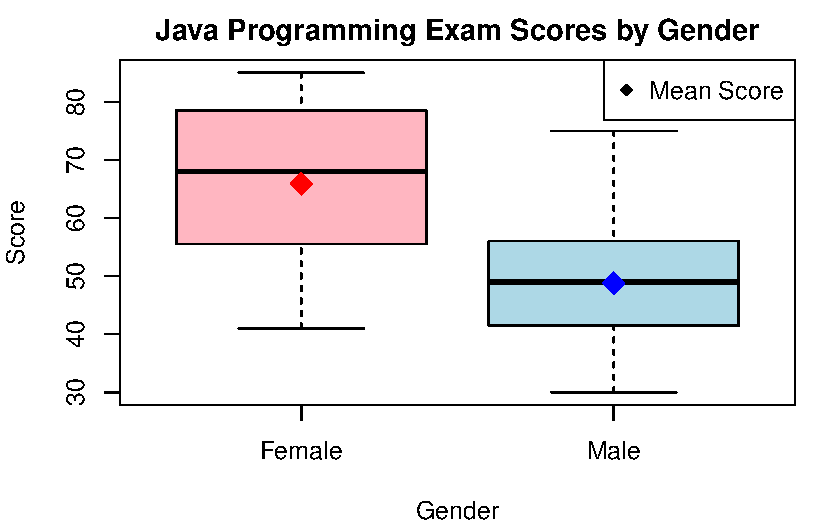
\includegraphics{Exercises1-1_files/figure-pdf/unnamed-chunk-6-1.pdf}

\section{Conclusion}\label{conclusion}

From our analysis, we can observe that female students (mean = r
round(mean(females), 2)) performed better on average than male students
(mean = r round(mean(males), 2)) in this Java programming examination.
The boxplot shows not only the difference in central tendency but also
the spread of scores within each group.




\end{document}
